
\section{Debugging and Profiling}

\subsection{Throughput and Latency}
In sequential programming measuring the performance of a program can be done through measuring its execution time.
This can be acheived by recording the time when the program starts and when it finishes, and calculating the difference.
The througput then becomes the

The impact of future optimizations can then be measured by comparing the execution times before and after the optimizations are applied.
As the number of tasks that can be solved in a given time is

However, in concurrent processing, execution times of individual instructions may overlap, making it challenging to calculate the execution time of the individual instructions \cite[21]{volkovLatencyHiding2016}.
The same type for time measurements can still be performed, but i

Instead, metrics such as latency, throughput, and concurrency can be used to characterize the process.

For example, latency is the average time between the start and end times of individual items, while throughput is the number of items processed within a given time interval divided by the duration of the interval.
Concurrency is the number of items processed simultaneously and can be measured at different moments in time or as an average over a particular interval.

\subsection{Creating Minimal Testing Example}
Wen debugging and profiling real-time applications it is often b

Beyond this the use of coroutines offers more control over the execution of the program, at the cost of requiring more thought to be put into the design of the program to avoid blocking the event loop.



\subsubsection{Profiling}
Profiling is the process of measuring the performance of a program, and is an important tool for optimizing programs.

In many cases it is straight forward; record the time when a task is started and when it is finished, and calculate the difference.


However, when working with heterogeneous computing systems, it is not always

nsys memory profiling does not work in Pinned Memory

\subsection{Nsight Compute}
\begin{figure}[H]
    \centering
    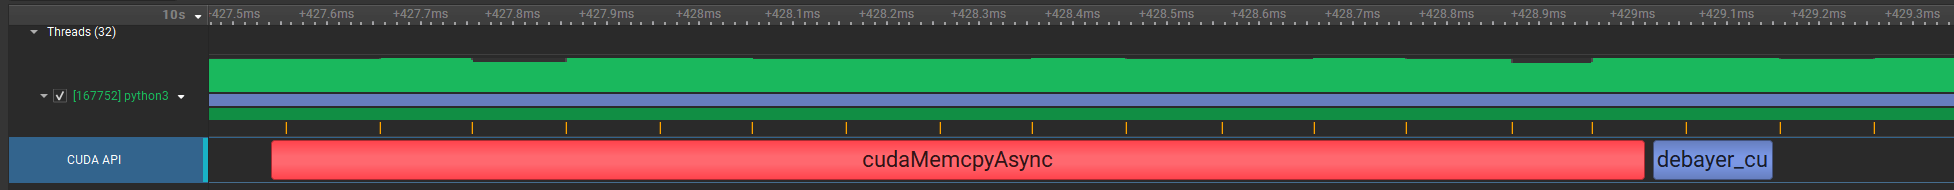
\includegraphics[width=\textwidth]{figures/memory_comparaison.png}
\end{figure}


% \begin{listing}[H]
%     \begin{minted}{python}
%         import asyncio, threading, time

%         def do_nothing(): pass
%         async def do_nothing_async(): pass

%         async def test_asyncio():
%             start_time = time.perf_counter()
%             await asyncio.gather(*[do_nothing_async() for _ in range(10000)])
%             end_time = time.perf_counter()
%             print(f"Asyncio took {end_time - start_time:.6f} seconds to complete.")

%         def test_threads():
%             threads = [threading.Thread(target=do_nothing) for _ in range(10000)]
%             start_time = time.perf_counter()
%             for thread in threads:
%                 thread.start()
%             for thread in threads:
%                 thread.join()
%             end_time = time.perf_counter()
%             print(f"Threads took {end_time - start_time:.6f} seconds to complete.")

%         if __name__ == "__main__":
%             asyncio.run(test_asyncio())
%             test_threads()
%     \end{minted}
%     \begin{minted}{bash}
%         >>> Asyncio took 0.311703 seconds to complete.
%         >>> Threads took 11.898036 seconds to complete.
%     \end{minted}
%     \caption{Comparison of asyncio and threads running on INTEL i7-11800H @ 2.30GHz.}
% \end{listing}